\documentclass[a4paper,14pt]{extarticle}
\renewcommand{\baselinestretch}{1.5}

\usepackage{polyglossia}
\setdefaultlanguage{russian}
\setotherlanguage{english}
\hyphenpenalty=1200
\exhyphenpenalty=1200
\tolerance=1800
\emergencystretch=1.4em

\usepackage{fontspec}
\setmainfont{Times New Roman}
\setmonofont{Courier New}
\newfontfamily\cyrillicfonttt{Courier New}
\usepackage{csquotes}

\usepackage{geometry}
\geometry{
  top=20mm,
  bottom=20mm,
  left=30mm,
  right=15mm
}
\setlength{\parindent}{1.25cm}
\usepackage{setspace}
\onehalfspacing
\hfuzz=10pt
\sloppy

\usepackage{titlesec}
\titleformat{\section}[block]{\filcenter\bfseries\fontsize{16}{19}\selectfont}{\thesection}{1em}{}
\titleformat{\subsection}[block]{\bfseries\normalsize}{\thesubsection}{1em}{}
\renewcommand{\thesection}{\arabic{section}}
\renewcommand{\thesubsection}{\arabic{section}.\arabic{subsection}}

\usepackage{tocloft}
\renewcommand{\cftsecleader}{\cftdotfill{\cftdotsep}}
\addto\captionsrussian{\renewcommand{\contentsname}{%
   {\centering\bfseries\fontsize{16}{19}\selectfont СОДЕРЖАНИЕ\par}
}}
\renewcommand{\cftsecaftersnum}{}
\renewcommand{\cftsubsecaftersnum}{.}

\usepackage{graphicx}
\usepackage[labelsep=endash]{caption}
\usepackage{float}
\usepackage{booktabs}
\usepackage{longtable}
\usepackage{array}
\usepackage{xurl}
\usepackage{tikz}
\usetikzlibrary{arrows.meta, positioning, shapes.geometric}
\addto\captionsrussian{\renewcommand{\figurename}{Рисунок}}
\addto\captionsrussian{\renewcommand{\tablename}{Таблица}}
\captionsetup[figure]{justification=centering}
\captionsetup[table]{justification=raggedright, singlelinecheck=false}

\usepackage[hidelinks]{hyperref}
\usepackage[
    backend=biber,
    style=gost-numeric,
    language=auto,
    sorting=none,
    autolang=other
]{biblatex}
\DeclareDelimFormat{multicitedelim}{\addcomma\space}
\addbibresource{report.bib}

\usepackage{enumitem}
\usepackage{indentfirst}
\usepackage{microtype}
\usepackage{amssymb}
\usepackage{amsmath}
\usepackage{siunitx}
\sisetup{output-decimal-marker={,}}

\newcolumntype{L}[1]{>{\raggedright\arraybackslash}p{#1}}
\newcolumntype{C}[1]{>{\centering\arraybackslash}p{#1}}
\setlist[itemize]{itemsep=0pt, topsep=0pt, parsep=0pt, partopsep=0pt, left=1.25cm}
\setlist[enumerate]{itemsep=0pt, topsep=0pt, parsep=0pt, partopsep=0pt, left=1.25cm, label=\arabic*., labelsep=0.5em}
\numberwithin{figure}{section}
\numberwithin{table}{section}

\newcommand{\appsection}[2]{%
  \clearpage
  \phantomsection
  \addcontentsline{toc}{section}{ПРИЛОЖЕНИЕ #1 --- #2}
  \begin{flushright}
  \bfseries Приложение #1
  \end{flushright}
  \begin{center}
  \bfseries #2
  \end{center}
}

\begin{document}
\pagestyle{empty}
\pagenumbering{gobble}

\begin{titlepage}
\thispagestyle{empty}
\begin{center}
    {\fontsize{14}{17}\selectfont Министерство науки и высшего образования Российской Федерации\par}
    {\fontsize{14}{17}\selectfont ФЕДЕРАЛЬНОЕ ГОСУДАРСТВЕННОЕ АВТОНОМНОЕ ОБРАЗОВАТЕЛЬНОЕ УЧРЕЖДЕНИЕ ВЫСШЕГО ОБРАЗОВАНИЯ\par}
    {\fontsize{14}{17}\selectfont «Национальный исследовательский университет ИТМО»\par}
    {\fontsize{14}{17}\selectfont (Университет ИТМО)\par}
\end{center}

\vspace{0.55cm}

\begin{center}
    {\fontsize{14}{17}\selectfont Факультет программной инженерии и компьютерной техники\par}
\end{center}

\vspace{0.55cm}

\begin{center}
    {\normalsize Образовательная программа: Системное и прикладное программное обеспечение\par}
    {\normalsize Направление подготовки (специальность): 09.04.04 Программная инженерия\par}
    {\normalsize Наименование практики: Научно-исследовательская работа\par}
\end{center}

\vspace{1.2cm}

\begin{center}
{\bfseries\fontsize{16}{19}\selectfont О\;Т\;Ч\;Е\;Т\par}
\vspace{0.4em}
{\normalsize о научно-исследовательской работе\par}
\vspace{0.8em}
{\normalsize Тема задания:\par}
\vspace{0.3em}
{\bfseries\fontsize{14}{17}\selectfont Сравнительный анализ архитектурных решений\par
серверной платформы текстовой MMORPG}
\end{center}

\vspace{1.0cm}
\begin{flushleft}
Обучающийся Горинов Даниил Андреевич, № группы P4116\par
\vspace{0.45cm}
Руководитель практики от университета: Маркина Татьяна Анатольевна,\par
руководитель в ИТМО, ответственный за практику (куратор)\par
\end{flushleft}

\vspace{0.75cm}
\begin{flushright}
Дата 21.06.2026\par
\end{flushright}

\vfill
\begin{center}
    {\normalsize Санкт-Петербург\par}
    {\normalsize 2026}
\end{center}
\end{titlepage}

\clearpage
\pagestyle{plain}
\pagenumbering{arabic}
\setcounter{page}{2}

\begin{center}
    \tableofcontents
\end{center}

\newpage

\section*{СПИСОК СОКРАЩЕНИЙ И УСЛОВНЫХ ОБОЗНАЧЕНИЙ}
\phantomsection
\addcontentsline{toc}{section}{СПИСОК СОКРАЩЕНИЙ И УСЛОВНЫХ ОБОЗНАЧЕНИЙ}
\label{sec:abbreviations}

\begin{table}[H]
\centering
\caption*{Сокращения и условные обозначения}
\footnotesize
\setlength{\tabcolsep}{3pt}
\renewcommand{\arraystretch}{1.15}
\begin{tabular}{L{3.5cm} L{11.0cm}}
\toprule
Сокращение & Значение \\
\midrule
MMORPG & Massively Multiplayer Online Role-Playing Game; в отчёте рассматривается текстовая многопользовательская ролевая онлайн-игра с серверной обработкой команд, чата и игровых транзакций. \\
API & Программный интерфейс взаимодействия клиента, внешней платформы или worker-процесса с серверной платформой. \\
WebSocket & Двусторонний протокол realtime-взаимодействия, определённый RFC 6455~\cite{rfc6455}. \\
Outbox & Таблица исходящих доменных событий, записываемая в одной транзакции с изменением бизнес-состояния. \\
Inbox & Механизм фиксации идентификаторов входящих сообщений для защиты от повторной обработки callback и команд. \\
Saga & Последовательность локальных транзакций с явными состояниями, повторными попытками и компенсациями. \\
Pub/Sub & Модель публикации и подписки; в Redis Pub/Sub используется для краткоживущих live-уведомлений. \\
Streams & Redis Streams; журнал событий с возможностью чтения истории и восстановления после разрыва соединения. \\
Source of truth & Основной источник достоверного состояния; в работе эту роль для экономики и прогресса выполняет PostgreSQL. \\
DLQ & Dead-letter queue, очередь сообщений, которые не удалось обработать после допустимого числа попыток. \\
p50, p95, p99 & 50-й, 95-й и 99-й процентили задержки обработки команд в экспериментальном стенде. \\
\bottomrule
\end{tabular}
\end{table}

\section*{ХАРАКТЕРИСТИКА МЕСТА ПРОХОЖДЕНИЯ ПРАКТИКИ}
\phantomsection
\addcontentsline{toc}{section}{ХАРАКТЕРИСТИКА МЕСТА ПРОХОЖДЕНИЯ ПРАКТИКИ}
\label{sec:place}

Практика выполнялась в Университете ИТМО на факультете программной инженерии и компьютерной техники по образовательной программе «Системное и прикладное программное обеспечение» направления подготовки 09.04.04 «Программная инженерия». Практика имела научно-исследовательский характер и была связана с анализом предметной области, постановкой исследовательской задачи, сравнением архитектурных решений, разработкой экспериментального стенда и оформлением отчётных материалов.

Руководитель практики от университета --- Маркина Татьяна Анатольевна, руководитель в ИТМО, ответственный за практику (куратор). Профильная внешняя организация в задании не указана; поэтому местом прохождения практики является Университет ИТМО. Данная структура раздела сохранена, поскольку учебно-методическое пособие ИТМО включает характеристику места прохождения практики в состав отчёта~\cite{markina2020practice}.

\section{Введение}
\label{sec:intro}

Настоящий отчёт подготовлен по результатам научно-исследовательской работы на тему сравнительного анализа архитектурных решений серверной платформы текстовой MMORPG. Предметная область включает игровые системы, в которых основная нагрузка возникает не от графического рендеринга, а от обработки пользовательских команд, чата, realtime-уведомлений, внутриигровой экономики, повторных callback внешних платформ и фоновых процессов. Для таких систем существенны высокая нагрузка, отказоустойчивость, наблюдаемость, контролируемая стоимость эксплуатации и корректность бизнес-состояния.

Цель работы --- обоснованно определить архитектурную комбинацию для серверной платформы текстовой MMORPG, которая сохраняет корректность игрового состояния, поддерживает realtime-взаимодействие и допускает рост нагрузки без преждевременного перехода к избыточно распределённой архитектуре.

Для достижения цели были решены следующие задачи:
\begin{enumerate}
    \item проанализирована предметная область серверных платформ текстовых многопользовательских онлайн-игр в социальных сетях, мессенджерах и web-клиентах;
    \item определены объект, предмет, цель, задачи и границы исследования;
    \item сформированы критерии сравнения: масштабируемость, надёжность, производительность, сложность внедрения, стоимость эксплуатации и наблюдаемость;
    \item подобраны и систематизированы научные и индустриальные источники;
    \item исследованы event-driven architecture, Transactional Outbox/Inbox, Saga, WebSocket-инфраструктура, брокеры сообщений, кэширование, PostgreSQL и Redis;
    \item разработан самостоятельный экспериментальный стенд, опубликованный в репозитории~\cite{gorinov2026mmorpgstand};
    \item выполнены серии нагрузочных и fault-injection экспериментов;
    \item сформированы итоговая экспериментальная матрица, evidence trace и практические рекомендации.
\end{enumerate}

Методика работы построена как трассируемая цепочка: критерий сравнения --- сценарий стенда --- метрика --- результат --- вывод --- рекомендация. Это отличает итоговое сравнение от простой качественной матрицы: ключевые выводы в отчёте опираются на источники, реализованные сценарии стенда и проверенные экспериментальные артефакты. Оформление отчёта выполнено с учётом требований учебно-методического пособия Университета ИТМО по организации и проведению производственной практики магистрантов: титульный лист, содержание, список сокращений, характеристика места практики, введение, основная часть, заключение, список источников и приложения; формат A4, Times New Roman 14 пт, полуторный интервал, поля 30/15/20/20 мм~\cite{markina2020practice}.

\section{План-график выполнения работы}
\label{sec:schedule}

План-график приведён в таблице~\ref{tab:schedule}. Этапы 2--4 образуют содержательную основу исследования. Этап 5 связан с оформлением письменного отчёта и проверкой воспроизводимости материалов. Этап 6 относится к пост-отчётному оформлению отзыва руководителя в модуле «Практика».

\begin{table}[H]
\centering
\caption{План-график выполнения НИР}
\label{tab:schedule}
\scriptsize
\setlength{\tabcolsep}{2pt}
\renewcommand{\arraystretch}{1.13}
\begin{tabular}{L{0.8cm} L{2.3cm} L{4.8cm} L{5.3cm} L{2.0cm}}
\toprule
Этап & Срок & Содержание & Результат & Статус \\
\midrule
1 & 02.03.2026 & Инструктаж обучающегося по требованиям охраны труда, техники безопасности, пожарной безопасности и внутреннего трудового распорядка & Факт прохождения организационного инструктажа & Выполнено \\
2 & 03.03.2026--23.03.2026 & Анализ предметной области и постановка задачи исследования & Объект, предмет, цель, задачи, критерии анализа и обзор источников & Выполнено \\
3 & 24.03.2026--26.05.2026 & Исследование архитектурных решений и сравнительный анализ подходов & Сценарии стенда, экспериментальная матрица и обоснование архитектурной комбинации & Выполнено \\
4 & 27.05.2026--21.06.2026 & Верификация выводов и формирование рекомендаций & Проверенные источники, терминология, evidence trace, fault-сценарии и рекомендации & Выполнено \\
5 & 02.03.2026--21.06.2026 & Оформление отчётных документов & Письменный отчёт, приложения со вспомогательными материалами, сборка PDF & Выполнено \\
6 & 22.06.2026--27.06.2026 & Получение отзыва руководителя практики & Отзыв и оценка руководителя в модуле «Практика» & Пост-отчётный этап \\
\bottomrule
\end{tabular}
\end{table}

\section{Выполнение этапа 2: анализ предметной области и постановка задачи}
\label{sec:stage2}

\subsection{Предметная область}
Текстовая MMORPG представляет собой многопользовательскую систему, в которой пользователь взаимодействует с игровым миром через команды, сообщения, уведомления, кнопки интерфейса социальной сети или мессенджера. В отличие от графических онлайн-игр, такая система не требует постоянной синхронизации трёхмерной сцены, но предъявляет высокие требования к серверной логике: экономические операции должны быть транзакционными, чат должен доставляться с малой задержкой, состояние игрока должно восстанавливаться после сбоя, а повторный callback внешней платформы не должен приводить к повторному начислению валюты или предмета.

Исследования backend-архитектур MMOG показывают, что серверная часть многопользовательской игры должна совмещать persistence, сетевую доставку, масштабирование и контроль согласованности состояния~\cite{kasenides2019mmog,zhang2008persistence}. Работы по transaction models и consistency requirements для MMOG подчёркивают, что действия игроков конкурируют за игровые ресурсы, предметы, валюту и состояние мира, поэтому простая обработка сообщений без модели согласованности недостаточна~\cite{zhang2011transactions,palant2006consistency,li2004continuous,diao2013consistency}. С учётом этого сценарии серверной платформы разделены на классы, приведённые в таблице~\ref{tab:scenario-classes}.

\begin{table}[H]
\centering
\caption{Классы сценариев серверной платформы текстовой MMORPG}
\label{tab:scenario-classes}
\footnotesize
\setlength{\tabcolsep}{3pt}
\renewcommand{\arraystretch}{1.15}
\begin{tabular}{L{3.3cm} L{5.0cm} L{6.1cm}}
\toprule
Класс сценариев & Типичные операции & Архитектурное требование \\
\midrule
Игровые команды & перемещение по локациям, выполнение задания, получение награды & транзакционная фиксация состояния, идемпотентность повторной команды, аудит результата \\
Чат и сообщения & сообщения комнаты, личные сообщения, системные уведомления & realtime-доставка, fan-out активным клиентам, отделение transient-сообщений от критичного состояния \\
Экономика и инвентарь & списание валюты, покупка предмета, выдача награды, обмен & строгие инварианты, уникальные ключи, локальные транзакции, Saga для цепочек с компенсациями \\
Интеграции и callback & ответы внешней платформы, повторные webhook, отложенные задания & Inbox, correlation id, устойчивость к повторной доставке \\
Realtime-состояние & online presence, обновления интерфейса, reconnect клиента & WebSocket, heartbeat, backpressure, replay или snapshot после разрыва соединения \\
Фоновые процессы & начисление периодических наград, события мира, обработка очередей & Outbox, worker-пулы, метрики lag/retry/DLQ, безопасная остановка и повторный запуск \\
\bottomrule
\end{tabular}
\end{table}

\subsection{Объект, предмет, цель и задачи исследования}
Объект исследования --- серверные платформы текстовых MMORPG, рассчитанные на взаимодействие пользователей через социальные сети, мессенджеры и web-клиенты. Предмет исследования --- архитектурные паттерны и инфраструктурные решения, обеспечивающие обработку игровых событий, чата, realtime-взаимодействия и внутриигровых транзакций.

Цель исследования сформулирована во введении: определить архитектурную комбинацию, которая обеспечивает корректность критичного состояния, поддерживает realtime-доставку и остаётся реализуемой при росте нагрузки. Для достижения цели исследование должно было не только перечислить решения, но и проверить их поведение в сценариях, характерных для текстовой MMORPG: повторная доставка callback, сбой после публикации события, потеря ephemeral-сообщения, reconnect клиента, устаревший кэш и частичная экономическая операция.

\subsection{Критерии анализа и источниковая база}
Критерии сравнения заданы практическим заданием и уточнены для экспериментальной проверки. В таблице~\ref{tab:criteria-main} каждому критерию сопоставлены проверяемые сценарии и метрики стенда. Такой способ нужен для того, чтобы итоговые рекомендации были связаны с наблюдаемыми данными, а не только с общими характеристиками технологий.

\begin{table}[H]
\centering
\caption{Критерии сравнения и способ их проверки}
\label{tab:criteria-main}
\scriptsize
\setlength{\tabcolsep}{1.5pt}
\renewcommand{\arraystretch}{1.15}
\begin{tabular}{L{2.9cm} L{4.5cm} L{4.2cm} L{3.6cm}}
\toprule
Критерий & Содержание критерия & Сценарий стенда & Метрики \\
\midrule
Масштабируемость & способность увеличивать число команд, сообщений, worker-процессов и подключений & серии 100/500/1000 для sync, outbox и chat & throughput, error rate, stream length \\
Надёжность & устойчивость к повторам, падению relay, потере transient-сообщений, reconnect и stale cache & duplicate callback, publish-no-ack, Pub/Sub loss, WebSocket replay, Saga, cache stale & duplicates, outbox pending, replay received, stale, completed/compensated \\
Производительность & влияние решения на задержку и пропускную способность & latency-серии sync/outbox/chat & p50, p95, p99, throughput \\
Сложность внедрения & число компонентов, состояний, контрактов и worker-путей & реализованные компоненты стенда & component/state/contract count, Saga states \\
Стоимость эксплуатации & инфраструктурная и операционная цена решения & stateful-зависимости, retained history, backlog & Redis, PostgreSQL, worker, stream length, attempts \\
Наблюдаемость & возможность доказать или опровергнуть архитектурный вывод метрикой & \texttt{/metrics/summary}, CSV/JSON/PNG & backlog age, lag, duplicates, Saga duration, cache stale \\
\bottomrule
\end{tabular}
\end{table}

Источники использовались по принципу применимости к конкретному утверждению. Рецензируемые работы применялись для анализа MMOG persistence, consistency и transaction models~\cite{kasenides2019mmog,zhang2008persistence,zhang2011transactions,palant2006consistency,li2004continuous,diao2013consistency}. Книги и паттерны распределённых систем использовались для терминов и интеграционных решений~\cite{kleppmann2017ddia,hohpe2004eip,eipIdempotentReceiver,eipCorrelationIdentifier,vogels2009eventual}. RFC и официальные документации применялись для свойств конкретных технологий~\cite{rfc6455,redis2026streams,redis2026pubsub,postgres2026ha,postgres2026partitioning}. Индустриальные материалы Microsoft, Microservices.io, Event-Driven.io, InfoQ, Ably и WebSocket.org использовались для современных эксплуатационных практик~\cite{microsoft2026eventdriven,richardson2026outbox,dudycz2020outbox,microsoft2026saga,morling2021saga,ably2024websocket,oriordan2024websockets}. Русскоязычные публикации по WebSocket/Socket.IO использовались как дополнительная сверка терминологии realtime-приложений~\cite{alpatov2024socketio,fedulov2025websocket}.

\section{Выполнение этапа 3: исследование архитектурных решений и сравнительный анализ}
\label{sec:stage3}

\subsection{Предварительные архитектурные гипотезы}
Перед экспериментальной проверкой решения были распределены по ролям. PostgreSQL рассматривался как источник достоверного состояния для экономики, прогресса, инвентаря и аудита; Transactional Outbox --- как способ атомарно связать изменение состояния и исходящее событие; Inbox --- как защита от повторной доставки; Redis Streams --- как persisted event log для replay; Redis Pub/Sub --- как transient-канал live fan-out; WebSocket gateway --- как realtime-интерфейс клиента; Saga --- как механизм координации долгих экономических цепочек; cache-aside --- как ускорение чтения некритичных данных.

Эти роли согласуются с источниками: Outbox устраняет проблему двойной записи, но допускает повторную публикацию при сбое relay между publish и отметкой доставки~\cite{richardson2026outbox,dudycz2020outbox}; Pub/Sub не хранит историю для позднего подписчика~\cite{redis2026pubsub}; Redis Streams предоставляет журнал для чтения истории~\cite{redis2026streams}; WebSocket является транспортом realtime-обмена, но не заменяет источник истины или журнал событий~\cite{rfc6455,ably2024websocket}; Saga применяется для последовательности локальных транзакций с компенсациями~\cite{microsoft2026saga,morling2021saga}.

Предварительная гипотеза состояла в том, что серверная платформа текстовой MMORPG должна строиться как комбинация перечисленных решений, а не как выбор одного универсального брокера, одной базы данных или одного realtime-протокола. Архитектурная схема гипотезы приведена на рисунке~\ref{fig:architecture-main}.

\begin{figure}[H]
\centering
\begin{tikzpicture}[node distance=8mm and 8mm, every node/.style={font=\small}]
    \node[draw, rounded corners, align=center, text width=2.9cm] (client) {Клиенты\\соцсети\\мессенджеры};
    \node[draw, rounded corners, align=center, text width=2.9cm, right=of client] (gateway) {HTTP/API\\WebSocket\\gateway};
    \node[draw, rounded corners, align=center, text width=2.9cm, right=of gateway] (domain) {Доменная\\обработка\\команд};
    \node[draw, rounded corners, align=center, text width=2.9cm, right=of domain] (pg) {PostgreSQL\\source\\of truth};
    \node[draw, rounded corners, align=center, text width=2.9cm, below=of domain] (outbox) {Outbox\\Inbox};
    \node[draw, rounded corners, align=center, text width=2.9cm, below=of gateway] (redis) {Redis Streams\\Pub/Sub\\cache};
    \node[draw, rounded corners, align=center, text width=2.9cm, below=of outbox] (workers) {Workers\\Saga};
    \draw[-{Latex[length=3mm]}] (client) -- (gateway);
    \draw[-{Latex[length=3mm]}] (gateway) -- (domain);
    \draw[-{Latex[length=3mm]}] (domain) -- (pg);
    \draw[-{Latex[length=3mm]}] (domain) -- (outbox);
    \draw[-{Latex[length=3mm]}] (outbox) -- (workers);
    \draw[-{Latex[length=3mm]}] (workers) -- (redis);
    \draw[-{Latex[length=3mm]}] (redis) -- (gateway);
    \draw[-{Latex[length=3mm]}] (workers) -- (pg);
\end{tikzpicture}
\caption{Архитектурная комбинация, проверенная на исследовательском стенде}
\label{fig:architecture-main}
\end{figure}

\subsection{Экспериментальный стенд}
Для проверки гипотезы был разработан самостоятельный стенд, опубликованный в репозитории~\cite{gorinov2026mmorpgstand}. Стенд реализован на Go и Python, запускается через Docker Compose и включает PostgreSQL, Redis, backend, worker, WebSocket-проверку и Python runner. Стенд моделирует минимальную серверную платформу текстовой игры: команды игрока изменяют баланс золота; Inbox фиксирует идентификаторы входящих сообщений; Outbox сохраняет исходящие события; worker публикует события в Redis Streams и Pub/Sub; WebSocket-клиент проверяет replay; Saga-worker завершает или компенсирует покупку; cache-aside endpoint демонстрирует устаревшее чтение.

Стенд не претендует на моделирование всего промышленного кластера MMORPG. Его назначение --- воспроизвести причинные свойства архитектурных паттернов в контролируемой среде. Поэтому абсолютные значения latency и throughput трактуются как локальные экспериментальные значения, а не как универсальный benchmark. Достоверность выводов обеспечивается повторяемостью сценариев, фиксированным seed 4116, автоматической проверкой инвариантов и сохранением CSV/JSON/PNG-артефактов.

\begin{table}[H]
\centering
\caption{Сценарии экспериментального стенда}
\label{tab:experiment-design}
\scriptsize
\setlength{\tabcolsep}{1.5pt}
\renewcommand{\arraystretch}{1.12}
\begin{tabular}{L{2.6cm} L{4.5cm} L{3.6cm} L{4.0cm}}
\toprule
Сценарий & Что проверяется & Метрики & Артефакты \\
\midrule
sync transaction & базовая локальная транзакция PostgreSQL & p50/p95/p99, throughput, error rate & scenario runs, latency/throughput PNG \\
outbox transaction & запись Outbox и асинхронная публикация worker & p50/p95/p99, backlog, attempts & summary, outbox backlog PNG \\
chat fan-out & запись и доставка чатовых сообщений & latency, throughput, stream length & scenario runs \\
duplicate callback & повторная доставка одной команды & duplicates, final gold & summary \\
publish-no-ack & публикация события без отметки доставки & redis duplicates, pending backlog & reliability matrix PNG \\
pubsub loss & потеря сообщения для позднего подписчика & delivered flag & summary \\
cache stale & устаревшее cache-aside чтение & cached gold, actual gold & cache consistency PNG \\
saga & успешная и компенсированная покупка & completed, compensated, duration & saga outcomes PNG \\
websocket replay & восстановление событий после reconnect & replay received & summary \\
\bottomrule
\end{tabular}
\end{table}

\subsection{Результаты по производительности и масштабируемости}
Нагрузочная часть эксперимента выполнена 21.06.2026. Для сценариев \texttt{sync\_transaction}, \texttt{outbox\_transaction} и \texttt{chat\_fanout} использованы размеры нагрузки 100, 500 и 1000 операций; каждый размер выполнен 5 раз. Итоговые агрегированные значения приведены в таблице~\ref{tab:perf-main}. Ошибки во всех строках равны нулю, что важно для интерпретации throughput: серия не скрывает падения запросов за счёт уменьшения числа успешных операций.

\begin{table}[H]
\centering
\caption{Агрегированные результаты нагрузочных серий}
\label{tab:perf-main}
\scriptsize
\setlength{\tabcolsep}{2pt}
\renewcommand{\arraystretch}{1.12}
\begin{tabular}{L{3.0cm} C{1.1cm} C{1.1cm} C{1.5cm} C{1.5cm} C{1.5cm} C{1.8cm} C{1.3cm}}
\toprule
Сценарий & Нагрузка & Повт. & p50, мс & p95, мс & p99, мс & throughput, req/s & error rate \\
\midrule
chat fan-out & 100 & 5 & 0,314 & 0,605 & 0,946 & 762,32 & 0 \\
chat fan-out & 500 & 5 & 0,275 & 0,501 & 0,843 & 911,61 & 0 \\
chat fan-out & 1000 & 5 & 0,266 & 0,461 & 0,658 & 966,00 & 0 \\
outbox transaction & 100 & 5 & 0,470 & 0,832 & 0,965 & 741,05 & 0 \\
outbox transaction & 500 & 5 & 0,453 & 0,756 & 1,026 & 737,15 & 0 \\
outbox transaction & 1000 & 5 & 0,453 & 0,767 & 1,180 & 755,65 & 0 \\
sync transaction & 100 & 5 & 0,448 & 1,108 & 1,735 & 682,97 & 0 \\
sync transaction & 500 & 5 & 0,379 & 0,605 & 1,150 & 845,72 & 0 \\
sync transaction & 1000 & 5 & 0,373 & 0,602 & 0,816 & 858,67 & 0 \\
\bottomrule
\end{tabular}
\end{table}

Рисунки~\ref{fig:latency-main} и~\ref{fig:throughput-main} показывают тот же результат в графической форме. Для локального стенда все три класса обработки остались в субмиллисекундном диапазоне p95 при нагрузке 1000 операций. Это не означает, что промышленная система будет иметь такие же задержки; вывод другой: добавление Outbox в командный путь на данном стенде не привело к неконтролируемому росту latency, а backlog после обработки был закрыт. Следовательно, Outbox допустим для критичных доменных событий при обязательном мониторинге backlog и повторных попыток.

\begin{figure}[H]
\centering
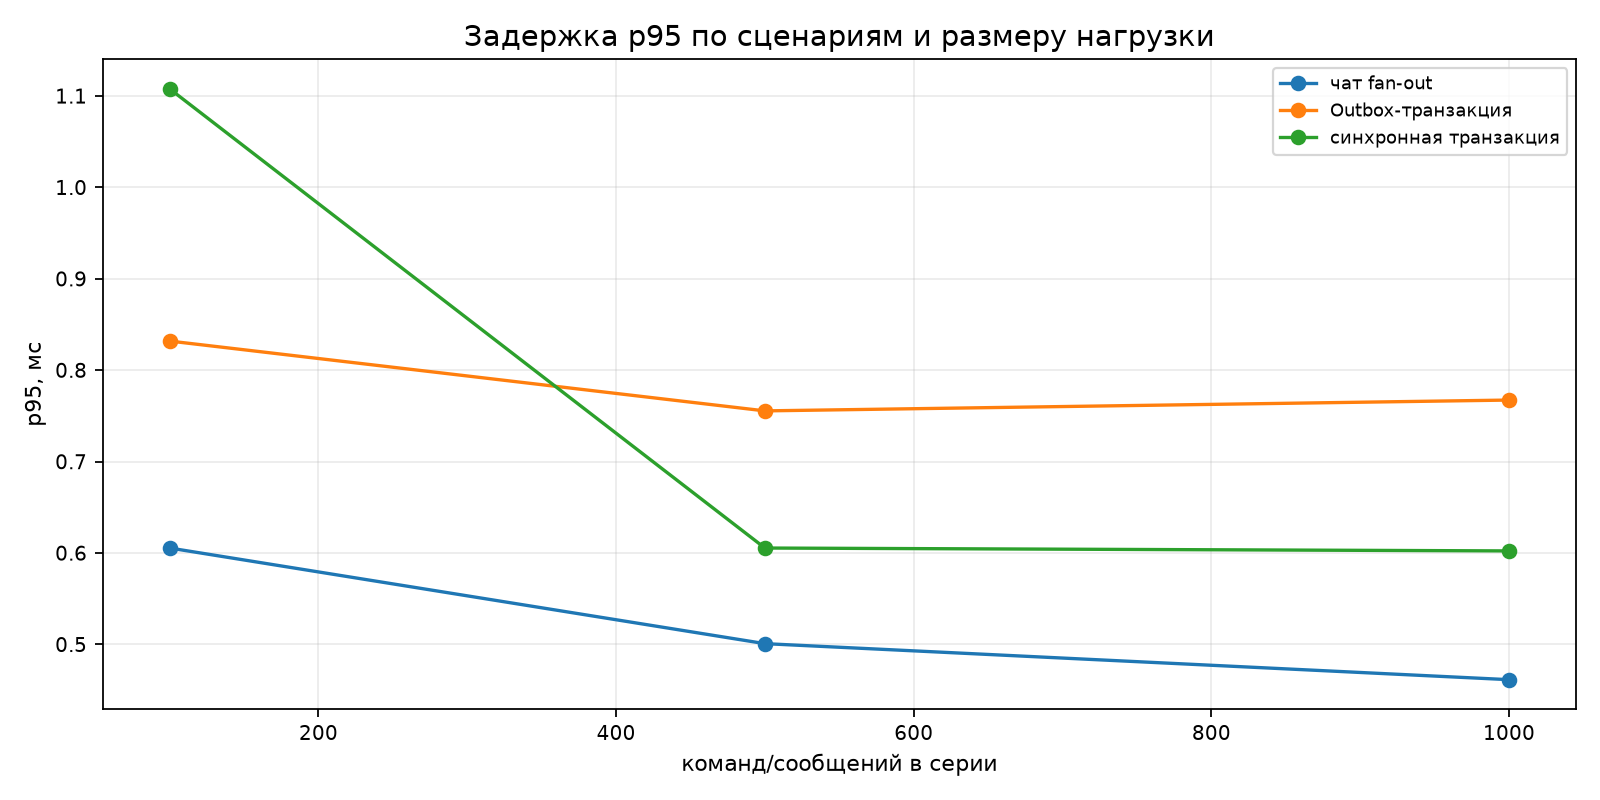
\includegraphics[width=0.92\textwidth]{../results/latest/latency_comparison.png}
\caption{Сравнение p95 latency по сценариям и размерам нагрузки}
\label{fig:latency-main}
\end{figure}

\begin{figure}[H]
\centering
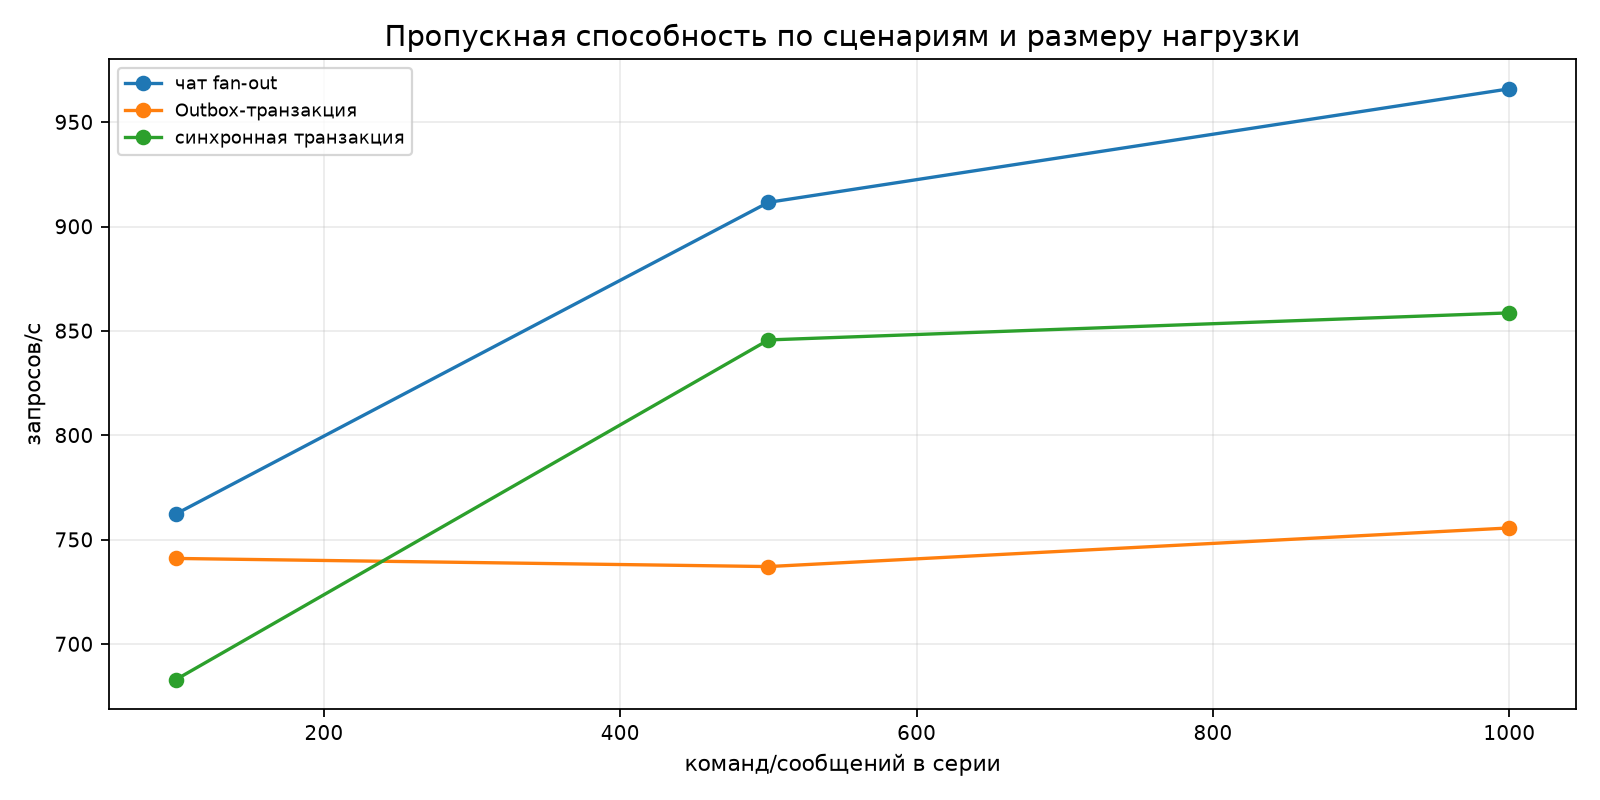
\includegraphics[width=0.92\textwidth]{../results/latest/throughput_comparison.png}
\caption{Сравнение throughput по сценариям и размерам нагрузки}
\label{fig:throughput-main}
\end{figure}

\subsection{Экспериментальная сравнительная матрица}
Итоговое сравнение построено по результатам \texttt{comparison\_matrix.csv}. Оценка от 1 до 5 отражает пригодность решения для задач текстовой MMORPG в проверенных условиях. Для производительности и масштабируемости использованы результаты нагрузочных серий; для надёжности --- fault-сценарии; для сложности внедрения, стоимости эксплуатации и наблюдаемости --- реализованные компоненты стенда, число состояний, stateful-зависимости и доступные метрики.

\begingroup
\scriptsize
\setlength{\tabcolsep}{1pt}
\renewcommand{\arraystretch}{1.12}
\begin{longtable}{L{2.5cm} C{0.75cm} C{0.75cm} C{0.75cm} C{0.75cm} C{0.75cm} C{0.75cm} C{0.75cm} L{3.1cm} L{3.3cm}}
\caption{Экспериментальная матрица сравнения архитектурных решений}
\label{tab:comparison-main} \\
\toprule
Решение & М & Н & П & СВ & СЭ & Набл. & Итог & Экспериментальное основание & Вывод \\
\midrule
\endfirsthead
\caption*{Продолжение таблицы \thetable{} --- Экспериментальная матрица сравнения архитектурных решений} \\
\toprule
Решение & М & Н & П & СВ & СЭ & Набл. & Итог & Экспериментальное основание & Вывод \\
\midrule
\endhead
\bottomrule
\endfoot
PostgreSQL transaction & 5 & 4 & 5 & 4 & 4 & 3 & 4,17 & p95=0,602 мс; throughput=858,67 req/s & подходит как source of truth, но не решает fan-out событий \\
Transactional Outbox & 5 & 5 & 5 & 3 & 3 & 5 & 4,33 & p95=0,767 мс; pending=0 & обеспечивает восстановимую публикацию после commit при worker и backlog-метриках \\
Inbox/idempotency & 5 & 5 & 5 & 4 & 5 & 4 & 4,67 & 5 повторов дали 4 дубля и один бизнес-результат & предотвращает повторный бизнес-эффект при повторной доставке \\
Redis Streams & 5 & 5 & 4 & 3 & 3 & 5 & 4,17 & stream\_len=8005; replay=3 & подходит для replay и контролируемой доставки, требует политики хранения \\
Redis Pub/Sub & 5 & 2 & 5 & 5 & 4 & 2 & 3,83 & late subscriber=false & пригоден для live fan-out, но не для durable-доставки критичного состояния \\
WebSocket gateway & 4 & 4 & 4 & 3 & 3 & 4 & 3,67 & WebSocket replay=3 & нужен для realtime-доставки, восстановление должно опираться на persisted stream \\
Saga orchestration & 3 & 5 & 3 & 2 & 2 & 5 & 3,33 & completed=1; compensated=1; p95=22,370 мс & подходит для долгих экономических цепочек с явными компенсациями \\
Cache-aside & 5 & 2 & 5 & 4 & 4 & 3 & 3,83 & cached=100; actual=150; stale=true & ускоряет чтение, но не может быть основанием экономических решений \\
Chat event fan-out & 5 & 4 & 5 & 4 & 4 & 4 & 4,33 & p95=0,461 мс; throughput=966,00 req/s & подходит для массовых сообщений при разделении Pub/Sub и stream history \\
\end{longtable}
\endgroup

Обозначения столбцов таблицы~\ref{tab:comparison-main}: М --- масштабируемость, Н --- надёжность, П --- производительность, СВ --- сложность внедрения, СЭ --- стоимость эксплуатации, Набл. --- наблюдаемость. Тепловая карта оценок по всем компонентам приведена на рисунке~\ref{fig:criteria-main}. Наибольший итоговый балл получил Inbox/idempotency, что отражает критичность защиты от повторного бизнес-эффекта в системах с внешними callback. Outbox и chat fan-out имеют одинаковый высокий итоговый балл, но решают разные задачи: первый связан с восстановимой публикацией событий, второй --- с массовой realtime-доставкой.

\begin{figure}[H]
\centering
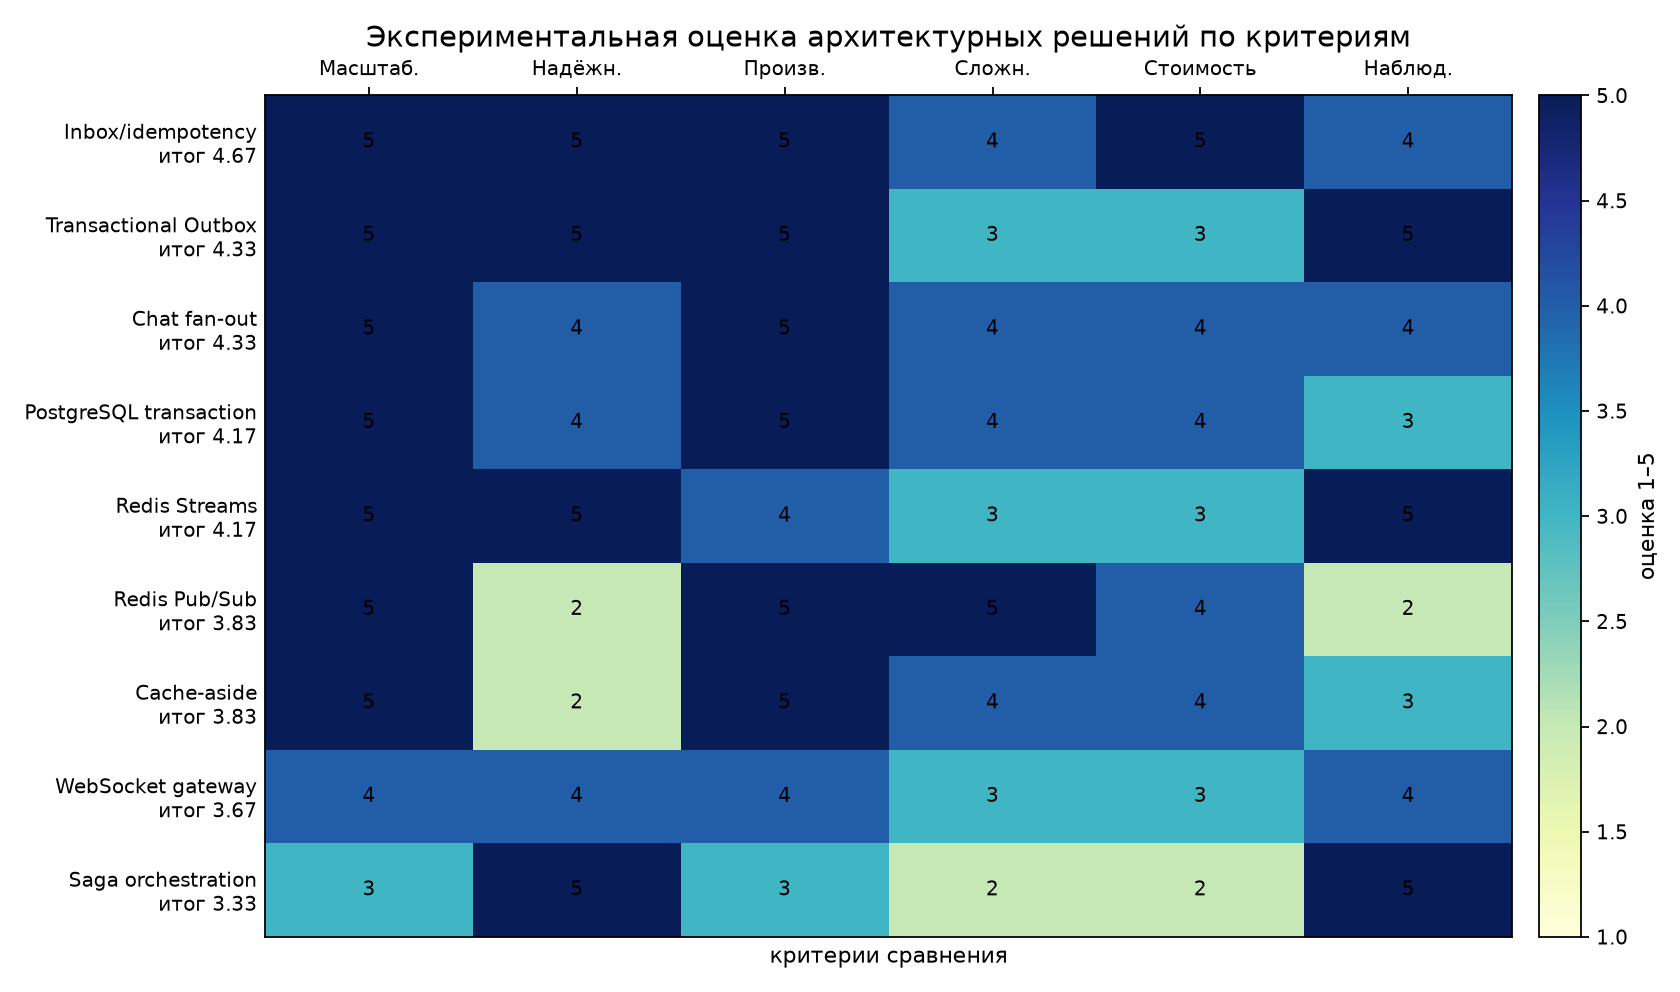
\includegraphics[width=0.98\textwidth]{../results/latest/criteria_radar.png}
\caption{Экспериментальная тепловая карта оценок архитектурных компонентов по критериям}
\label{fig:criteria-main}
\end{figure}

\subsection{Обоснование архитектурной комбинации}
На основании источников и эксперимента обоснована следующая архитектурная комбинация.

PostgreSQL должен оставаться источником истины для экономики, прогресса, инвентаря и аудита. Это следует из требований к локальным ACID-транзакциям, уникальным ограничениям и восстановлению состояния~\cite{postgres2026ha,postgres2026partitioning}. Экспериментальная серия показала, что локальная транзакционная обработка обеспечивает устойчивую базовую задержку и нулевой error rate на стенде, но сама по себе не решает доставку событий внешним потребителям.

Transactional Outbox следует использовать для доменных событий, связанных с изменением состояния. Эксперимент \texttt{publish\_no\_ack} воспроизвёл транспортный дубль: событие было опубликовано, но отметка доставки не была зафиксирована, после чего worker повторил публикацию. Это подтверждает известное ограничение Outbox: паттерн устраняет двойную запись, но не отменяет требования к идемпотентным потребителям~\cite{dudycz2020outbox,eipIdempotentReceiver}. Поэтому Outbox должен применяться вместе с Inbox, уникальными ключами и дедупликацией на стороне потребителя.

Redis Pub/Sub и Redis Streams должны использоваться совместно, но для разных гарантий. Pub/Sub подходит для live fan-out активным WebSocket-шлюзам, поскольку имеет малую задержку и простую модель подписки; при этом сценарий \texttt{pubsub\_loss} подтвердил, что поздний подписчик не получает уже опубликованное сообщение. Redis Streams, напротив, хранит события и обеспечивает replay: WebSocket-проверка получила 3 события после подключения с начальным \texttt{last=0-0}. Следовательно, критичное состояние восстанавливается не из Pub/Sub, а из PostgreSQL или persisted stream.

Saga-оркестрация оправдана для долгих экономических цепочек, где несколько локальных транзакций должны завершиться согласованным финалом. На стенде были получены оба наблюдаемых исхода: \texttt{completed=1} и \texttt{compensated=1}. При этом Saga имеет более высокую сложность внедрения и эксплуатации, поэтому не должна заменять простые локальные транзакции для обычных команд.

Cache-aside допустим только для данных, где устаревшее чтение не нарушает экономические инварианты. Сценарий \texttt{cache\_stale} зафиксировал расхождение \texttt{cached=100} и \texttt{actual=150}; значит, кэш не может быть основанием для решений о списании валюты, выдаче предметов или правах владения.

\section{Выполнение этапа 4: верификация выводов и формирование рекомендаций}
\label{sec:stage4}

\subsection{Матрица отказов и проверка надёжности}
Верификация выводов выполнялась по fault-сценариям, которые соответствуют типичным отказам серверной платформы текстовой MMORPG: повторная доставка callback, падение relay после publish, потеря transient-сообщения, reconnect клиента, stale cache и частичная Saga. Результаты приведены в таблице~\ref{tab:fault-main}; графическое представление --- на рисунках~\ref{fig:reliability-main}--\ref{fig:saga-main}.

\begin{table}[H]
\centering
\caption{Результаты fault-injection сценариев}
\label{tab:fault-main}
\footnotesize
\setlength{\tabcolsep}{2pt}
\renewcommand{\arraystretch}{1.12}
\begin{tabular}{L{3.0cm} L{4.8cm} L{3.7cm} L{3.4cm}}
\toprule
Сценарий & Результат & Проверенный вывод & Архитектурное следствие \\
\midrule
Duplicate callback & 5 запросов; 4 дубля; итоговый баланс 7 & повторная доставка не изменила состояние повторно & обязателен Inbox/idempotency key \\
Publish-no-ack & redis duplicates: 1; outbox pending: 0 & транспортный дубль возможен, backlog закрывается & нужны идемпотентные потребители и outbox monitoring \\
Pub/Sub late subscriber & delivered=false & поздний подписчик не получает историю & Pub/Sub нельзя использовать как durable-журнал \\
WebSocket replay & received=3 & reconnect восстанавливает события из stream & нужен last-seen marker и persisted stream \\
Cache stale & cached=100; actual=150; stale=true & cache-aside может вернуть устаревшее значение & кэш не является source of truth для экономики \\
Saga outcomes & completed=1; compensated=1; p95=22,370 мс & оба исхода наблюдаемы и проверяемы & Saga требует явных состояний и компенсаций \\
\bottomrule
\end{tabular}
\end{table}

\begin{figure}[H]
\centering
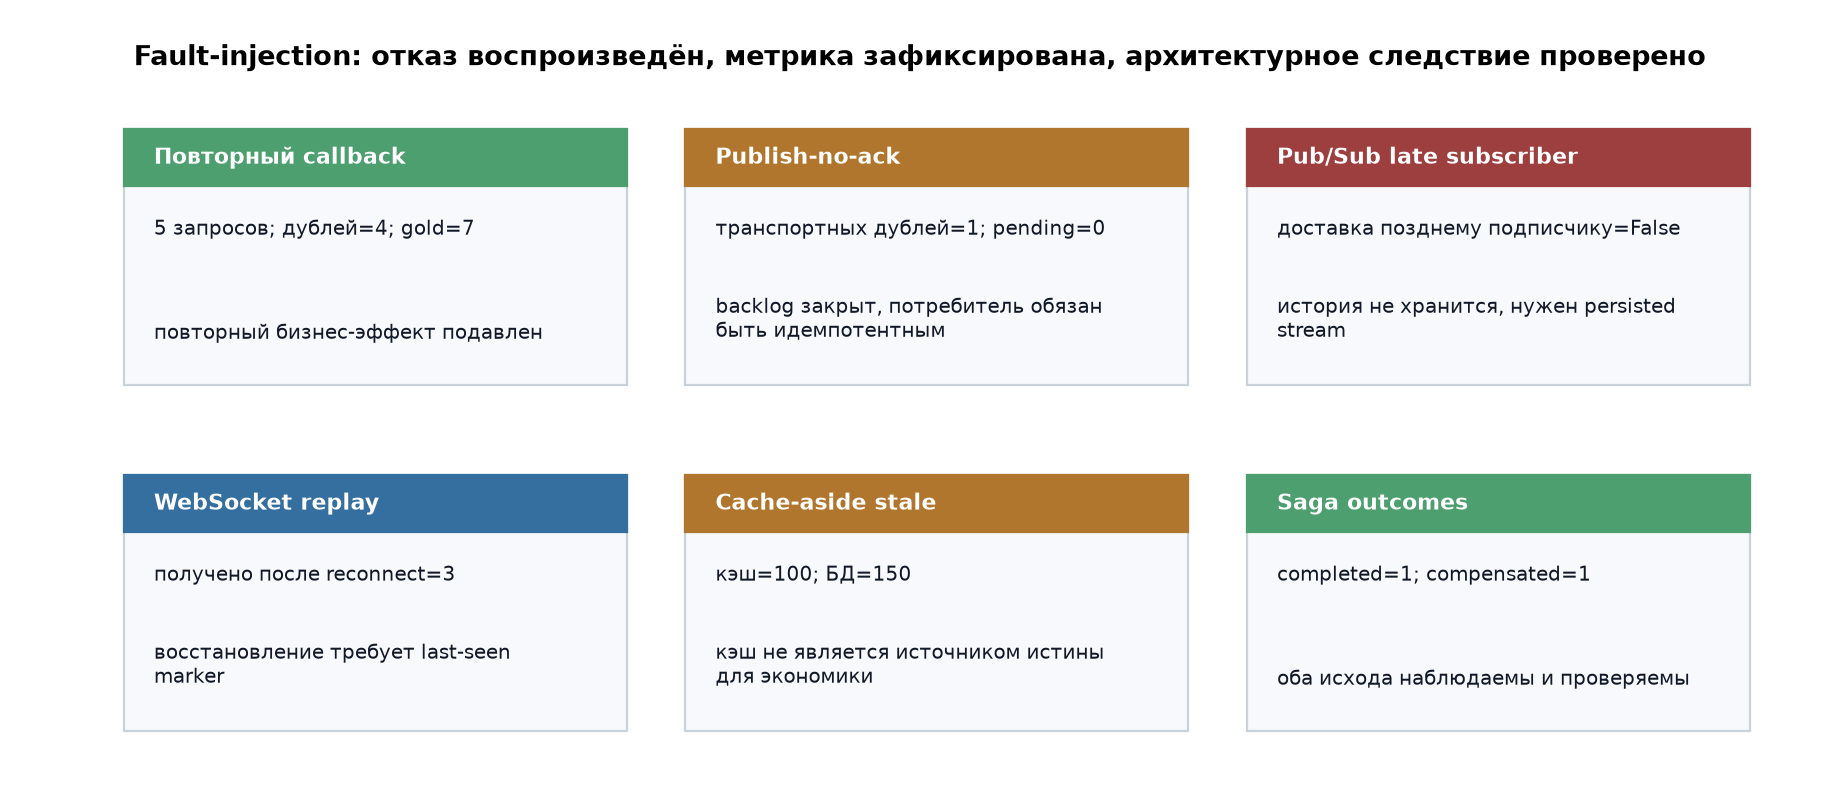
\includegraphics[width=0.98\textwidth]{../results/latest/reliability_matrix.png}
\caption{Матрица fault-injection проверок с наблюдаемыми значениями}
\label{fig:reliability-main}
\end{figure}

\begin{figure}[H]
\centering
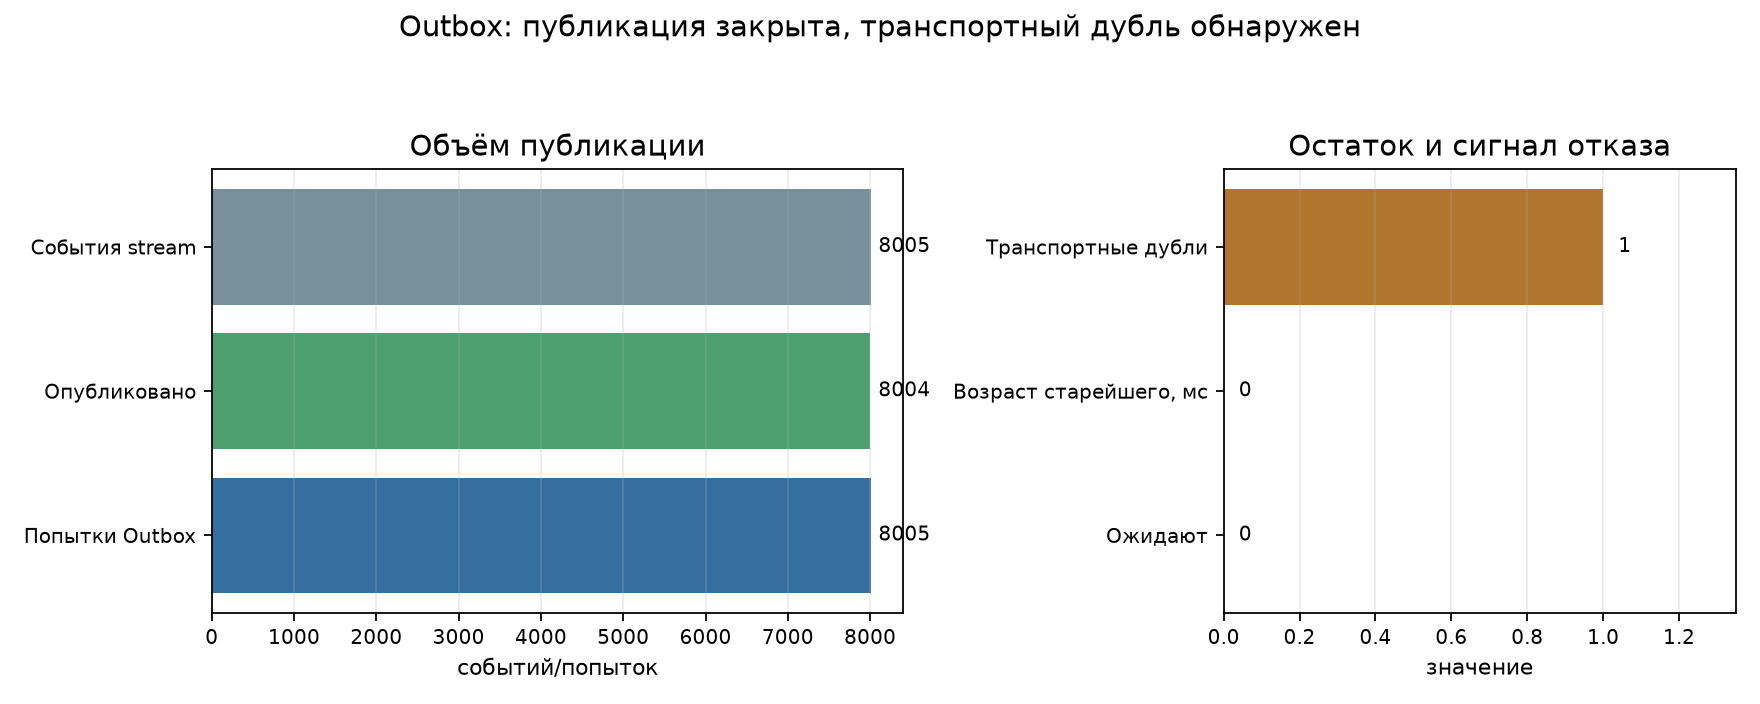
\includegraphics[width=0.92\textwidth]{../results/latest/outbox_backlog.png}
\caption{Раздельная проверка объёма Outbox/Streams и остаточного backlog}
\label{fig:outbox-main}
\end{figure}

\begin{figure}[H]
\centering
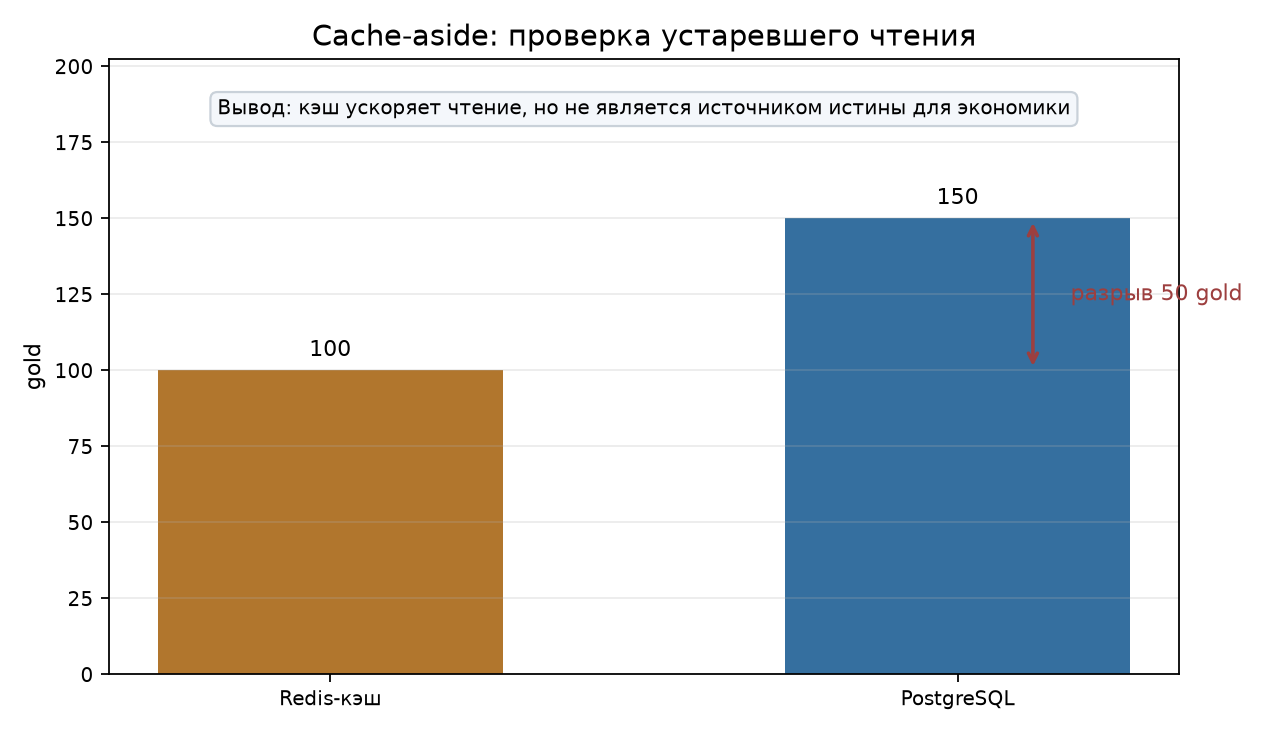
\includegraphics[width=0.82\textwidth]{../results/latest/cache_consistency.png}
\caption{Cache-aside: расхождение между кэшем и source of truth}
\label{fig:cache-main}
\end{figure}

\begin{figure}[H]
\centering
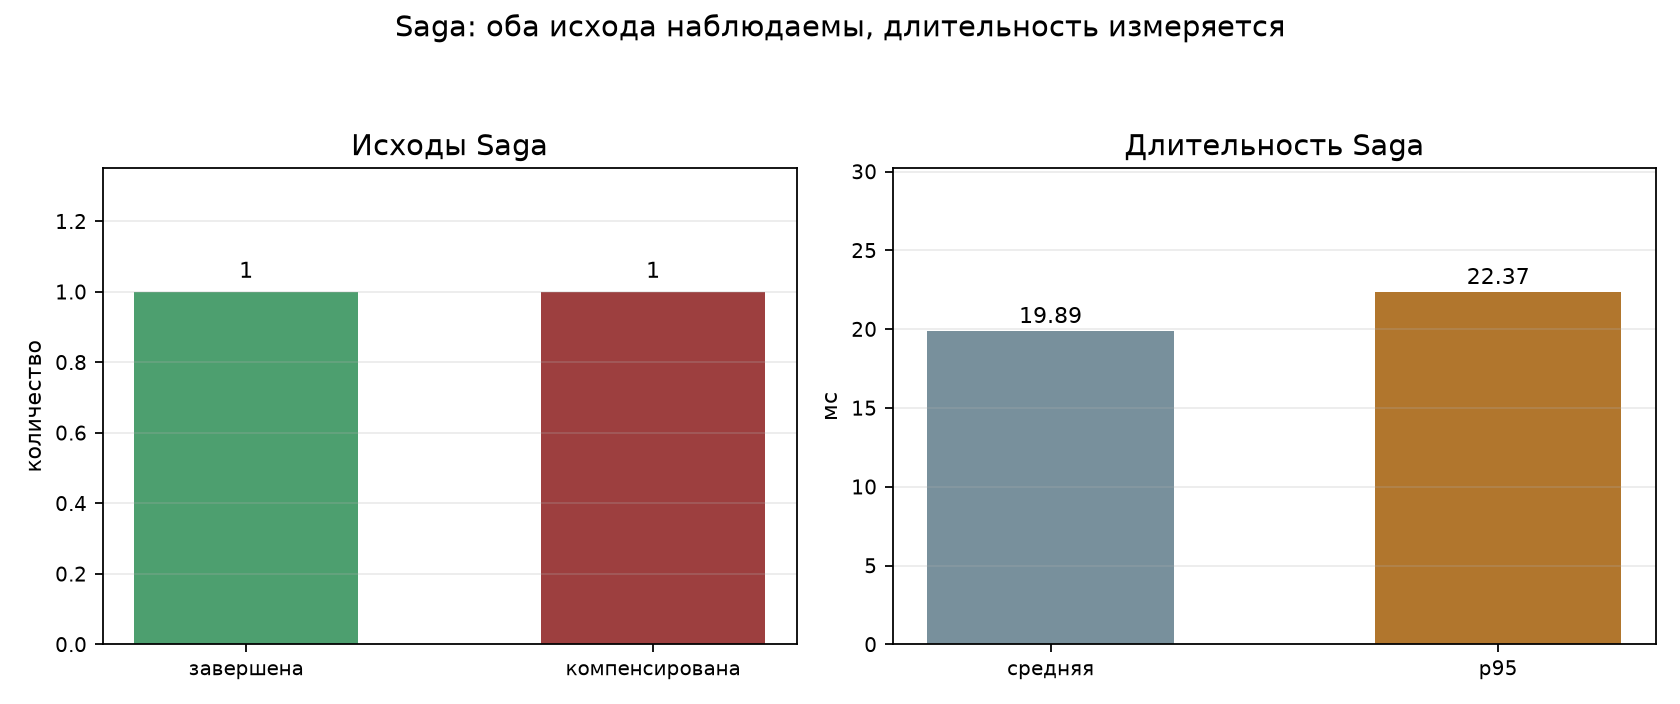
\includegraphics[width=0.92\textwidth]{../results/latest/saga_outcomes.png}
\caption{Saga: исходы и длительность выполнения}
\label{fig:saga-main}
\end{figure}

Содержательный результат fault-injection состоит в том, что каждый проверяемый отказ не просто воспроизведён, но связан с проектным решением. Повторная доставка callback требует Inbox; publish-no-ack требует идемпотентных потребителей; Pub/Sub loss требует persisted stream или восстановления из PostgreSQL; WebSocket reconnect требует last-seen marker; stale cache требует запрета на использование кэша как источника экономических решений; Saga требует явных состояний и компенсаций.

\subsection{Evidence trace}
Для исключения разрыва между экспериментом и рекомендациями сформирована evidence trace: каждому критерию сопоставлены сценарий, метрика, артефакт, результат и вывод. Сводная версия приведена в таблице~\ref{tab:evidence-main}; полная JSON-форма сохранена в \texttt{results/latest/evidence\_trace.json}.

\begingroup
\scriptsize
\setlength{\tabcolsep}{1.5pt}
\renewcommand{\arraystretch}{1.12}
\begin{longtable}{L{2.8cm} L{3.1cm} L{3.1cm} L{3.4cm} L{2.9cm}}
\caption{Трассировка доказательств от критерия к выводу}
\label{tab:evidence-main} \\
\toprule
Критерий & Сценарий & Метрика & Артефакт & Вывод \\
\midrule
\endfirsthead
\caption*{Продолжение таблицы \thetable{} --- Трассировка доказательств от критерия к выводу} \\
\toprule
Критерий & Сценарий & Метрика & Артефакт & Вывод \\
\midrule
\endhead
\bottomrule
\endfoot
Масштабируемость & серии 100/500/1000 для sync/outbox/chat & throughput и error rate & scenario runs, throughput PNG & горизонтально масштабируемые каналы нужны прежде всего для fan-out и worker-обработки событий \\
Надёжность & duplicate, publish-no-ack, Pub/Sub loss, replay, cache, Saga & duplicates, pending, delivered, stale, completed/compensated & summary, reliability matrix PNG & надёжность достигается комбинацией Outbox, Inbox, Streams, Saga и source of truth \\
Производительность & latency и throughput серии & p50, p95, p99, throughput & latency и throughput PNG & overhead Outbox приемлем только при контроле backlog и retries \\
Сложность внедрения & реализованные компоненты и state machine & число компонентов, состояний и контрактов & comparison matrix CSV & сложные паттерны применяются только там, где локальная транзакция не закрывает риск \\
Стоимость эксплуатации & stateful-зависимости и retained history & stream length, attempts, worker, PostgreSQL, Redis & comparison matrix CSV, backlog PNG & стоимость определяется политикой хранения stream/outbox и наблюдаемостью worker \\
Наблюдаемость & \texttt{/metrics/summary} и артефакты & backlog age, duplicates, Saga duration, cache stale & summary, evidence trace JSON & рекомендация считается проверенной только при наличии наблюдаемой метрики \\
\end{longtable}
\endgroup

\subsection{Наблюдаемость и проверяемые метрики}
Для архитектуры серверной платформы текстовой MMORPG наблюдаемость является не вспомогательным свойством, а условием управляемости. Если система не измеряет возраст Outbox backlog, число повторных публикаций, stream lag, длительность Saga и устаревшие значения кэша, то эксплуатационная команда не сможет отличить корректную повторную доставку от потери события или зависшего worker. В стенде эта связь отражена через endpoint \texttt{/metrics/summary}; ключевые метрики приведены в таблице~\ref{tab:observability-main}.

\begin{table}[H]
\centering
\caption{Метрики наблюдаемости, использованные в исследовании}
\label{tab:observability-main}
\scriptsize
\setlength{\tabcolsep}{1.5pt}
\renewcommand{\arraystretch}{1.12}
\begin{tabular}{L{5.2cm} L{2.0cm} L{6.9cm}}
\toprule
Метрика & Значение в запуске & Что подтверждает \\
\midrule
\texttt{inbox\_count} & 16003 & команды и callback фиксируются для дедупликации \\
\texttt{outbox\_published} & 8004 & worker реально публиковал исходящие события \\
\texttt{outbox\_attempts\_total} & 8005 & повторная попытка после publish-no-ack наблюдаема \\
\texttt{outbox\_pending} & 0 & backlog закрыт после завершения эксперимента \\
\texttt{outbox\_oldest\_pending\_ms} & 0 & незакрытых старых событий нет \\
\texttt{redis\_stream\_len} & 8005 & persisted stream содержит историю для replay \\
\texttt{redis\_duplicate\_events} & 1 & транспортный дубль воспроизведён и измерен \\
\texttt{chat\_messages} & 8000 & чатовая нагрузка обработана полностью \\
\texttt{chat\_stream\_len} & 8000 & чатовые события сохранены в stream \\
\texttt{saga\_completed} / \texttt{saga\_compensated} & 1 / 1 & оба исхода Saga достигнуты \\
\texttt{saga\_duration\_p95\_ms} & 22,370 & длительность Saga наблюдаема \\
\bottomrule
\end{tabular}
\end{table}

\subsection{Проверка терминологии, источников и ограничений валидности}
Терминология была уточнена по уровням гарантий. At-least-once означает возможную повторную доставку сообщения. Идемпотентность означает отсутствие дополнительного побочного эффекта при повторной обработке. Однократный бизнес-результат достигается за счёт уникальных ключей, транзакционных ограничений, Inbox и дедупликации, а не за счёт абсолютной гарантии транспорта. Такая формулировка согласуется с паттерном Idempotent Receiver и описаниями delivery guarantees для Outbox/Inbox~\cite{dudycz2020outbox,eipIdempotentReceiver,kleppmann2017ddia}.

Проверка источников включала сверку URL/DOI, авторства, года публикации и применимости источника к утверждению. Дата обращения для электронных источников --- 21.06.2026. Если HTML-страница источника возвращала 403 при автоматизированной проверке, библиографические сведения сверялись по DOI-метаданным Crossref; такой источник сохранялся, если DOI и описание публикации подтверждались.

Ограничения валидности зафиксированы отдельно. Во-первых, стенд проверяет архитектурные свойства, а не поведение полного production-кластера с геораспределением, реальной авторизацией, платежами и миллионами WebSocket-подключений. Во-вторых, локальные latency и throughput зависят от машины, Docker и фоновой нагрузки, поэтому используются как воспроизводимые значения конкретного стенда. Во-третьих, оценки сложности внедрения и стоимости эксплуатации опираются на реализованные компоненты стенда и источники; при переходе к промышленной системе они должны уточняться с учётом требований к SLA, резервированию, хранению истории и мониторингу.

\subsection{Практические рекомендации}
Практические рекомендации приведены в таблице~\ref{tab:recommendations-main}. Каждая рекомендация связана с экспериментальным основанием или источником; рекомендации без проверяемого основания в итоговый набор не включались.

\begin{table}[H]
\centering
\caption{Практические рекомендации по проектированию платформы}
\label{tab:recommendations-main}
\footnotesize
\setlength{\tabcolsep}{2pt}
\renewcommand{\arraystretch}{1.12}
\begin{tabular}{L{0.9cm} L{5.8cm} L{3.8cm} L{4.4cm}}
\toprule
№ & Рекомендация & Основание & Доказательное значение \\
\midrule
R1 & PostgreSQL использовать как source of truth для экономики, инвентаря, прогресса и аудита & sync-серии, cache stale, документация PostgreSQL & кэш вернул 100 при фактическом значении 150; критичное решение должно идти в БД \\
R2 & Каждую внешнюю команду и callback снабжать idempotency key и фиксировать в Inbox & duplicate callback, Idempotent Receiver & 5 повторов дали один бизнес-результат и 4 зарегистрированных дубля \\
R3 & Исходящие доменные события публиковать через Transactional Outbox и проектировать потребителей идемпотентными & publish-no-ack, Outbox/Inbox sources & транспортный дубль появился, но \texttt{outbox\_pending}=0 после повторной обработки \\
R4 & Redis Pub/Sub использовать только для transient fan-out, а Redis Streams --- для replay и контролируемой доставки & Pub/Sub loss, WebSocket replay, Redis docs & поздний подписчик не получил сообщение; WebSocket replay получил 3 события \\
R5 & Saga применять только для долгих экономических операций с явными компенсациями & Saga scenario, Microsoft/InfoQ & получены оба исхода: completed=1 и compensated=1 \\
R6 & В мониторинг включить backlog age, stream lag, duplicates, Saga duration, cache stale и error rate & \texttt{/metrics/summary}, evidence trace & без этих метрик невозможно доказательно связать отказ с архитектурной причиной \\
\bottomrule
\end{tabular}
\end{table}

\section{Выполнение этапа 5: оформление отчётных документов}
\label{sec:stage5}

Этап 5 выполнялся в течение всего периода НИР с 02.03.2026 по 21.06.2026 и завершился подготовкой письменного отчёта. По заданию на практику в основной части должны быть подробно описаны этапы 2--4, а в приложениях размещены результаты данных этапов. В настоящем отчёте ключевые интерпретированные результаты --- сравнительная матрица, графики, таблица метрик, evidence trace и рекомендации --- вынесены в основную часть, поскольку на них непосредственно ссылается текст и по ним проводится доказательное сравнение. В приложениях оставлены вспомогательные материалы: команды запуска, структура стенда, перечень raw-артефактов и протокол проверки.

Оформление выполнено в соответствии с методическим пособием ИТМО~\cite{markina2020practice}: сохранены титульный лист, содержание, список сокращений, характеристика места практики, введение, основная часть, заключение, список источников и приложения. Отчёт собирается командой \texttt{./build\_pdf.sh}; сборка проверяется по отсутствию ошибок LaTeX, неопределённых ссылок и неопределённых цитирований. Экспериментальные артефакты создаются командами \texttt{make experiment} и \texttt{make verify-results}; полные команды и структура стенда приведены в приложении~\ref{app:repo}.

\section{Заключение}
\label{sec:conclusion}

В ходе научно-исследовательской работы выполнены этапы 2--5 задания на практику. На этапе 2 проанализирована предметная область серверных платформ текстовых MMORPG, определены объект, предмет, цель, задачи, классы сценариев, критерии анализа и источниковая база. На этапе 3 исследованы архитектурные решения и разработан практический стенд, на котором выполнены серии 100/500/1000 операций для sync/outbox/chat и fault-сценарии для duplicate callback, publish-no-ack, Pub/Sub loss, WebSocket replay, stale cache и Saga. На этапе 4 выводы верифицированы через источники, терминологию, матрицу отказов, evidence trace и проверяемые метрики. На этапе 5 подготовлен письменный отчёт и приложения со вспомогательными материалами.

Цель работы достигнута: обоснована архитектурная комбинация PostgreSQL + Transactional Outbox/Inbox + Redis Streams/Pub/Sub + WebSocket gateway + Saga + cache-aside с разграничением областей применения. PostgreSQL используется как источник истины для критичного состояния; Outbox и Inbox обеспечивают восстановимую публикацию и защиту от повторного бизнес-эффекта; Redis Pub/Sub применяется только для transient fan-out, а Redis Streams --- для replay; WebSocket обеспечивает realtime-доставку при наличии механизма восстановления; Saga применяется к долгим экономическим цепочкам; cache-aside ограничивается данными, где допустима устарелость или есть проверка через source of truth.

Итоговые рекомендации подтверждены экспериментальными артефактами: \texttt{summary.json}, \texttt{scenario\_runs.csv}, \texttt{comparison\_matrix.csv}, \texttt{evidence\_trace.json}, графиками latency/throughput, матрицей надёжности, графиками Outbox backlog, cache consistency и Saga outcomes. Команда \texttt{make verify-results} проверяет наличие артефактов, структуру серий, отсутствие незакрытого Outbox backlog и выполнение ключевых инвариантов. Отзыв руководителя и оценка за практику оформляются руководителем в модуле «Практика» в период 22.06.2026--27.06.2026; в отчёте они не указываются как установленный факт.

\clearpage
\section{Список использованных источников}
\label{sec:bibliography}
\begingroup
\sloppy
\raggedright
\nocite{*}
\printbibliography[heading=none]
\endgroup

\appsection{1}{Репозиторий, команды запуска и структура стенда}
\label{app:repo}

Публичный репозиторий исследовательского стенда:
\begin{center}
\href{https://github.com/gorinovdan/mmorpg-architecture-research}{github.com/gorinovdan/mmorpg-architecture-research}
\end{center}

\begin{table}[H]
\centering
\caption*{Команды запуска и проверки стенда}
\footnotesize
\setlength{\tabcolsep}{3pt}
\renewcommand{\arraystretch}{1.15}
\begin{tabular}{L{5.0cm} L{9.6cm}}
\toprule
Команда & Назначение \\
\midrule
\texttt{make deps} & Создать Python-окружение и установить зависимости для графиков. \\
\texttt{make test} & Запустить Go-тесты, проверить Docker Compose и Python-скрипты. \\
\texttt{make up} & Собрать и поднять PostgreSQL, Redis, backend и worker. \\
\texttt{make migrate} & Проверить применение миграций backend при старте. \\
\texttt{make experiment} & Выполнить серии нагрузки и fault-injection сценарии. \\
\texttt{make verify-results} & Проверить инварианты, матрицы, графики и evidence trace. \\
\texttt{make down} & Остановить контейнеры стенда. \\
\bottomrule
\end{tabular}
\end{table}

\begin{table}[H]
\centering
\caption*{Структура стенда}
\footnotesize
\setlength{\tabcolsep}{3pt}
\renewcommand{\arraystretch}{1.15}
\begin{tabular}{L{6.2cm} L{8.4cm}}
\toprule
Путь & Назначение \\
\midrule
\url{cmd/researchd} & Backend и worker: HTTP API, WebSocket, PostgreSQL, Redis, Outbox, Inbox, Saga, cache-aside. \\
\url{cmd/wscheck} & Проверка WebSocket replay после подключения. \\
\url{internal/expstats} & Проверяемые функции расчёта процентилей и дублей. \\
\url{scripts/run_experiments.py} & Запуск сценариев нагрузки и отказов, сбор CSV/JSON/PNG. \\
\url{scripts/verify_results.py} & Проверка инвариантов, артефактов и evidence trace. \\
\url{docs/architecture.md} & Описание границ стенда, компонентов, потоков данных и метрик. \\
\url{docs/experiments.md} & Методика экспериментов, артефакты и правила интерпретации. \\
\url{.github/workflows/ci.yml} & GitHub Actions для Go-тестов, Docker smoke test и проверки артефактов. \\
\bottomrule
\end{tabular}
\end{table}

\appsection{2}{Raw-сводка экспериментальных артефактов}
\label{app:raw}

Приложение содержит сокращённую сводку исходных артефактов стенда. Интерпретация результатов приведена в основной части отчёта; здесь зафиксированы файлы, по которым проверяется воспроизводимость.

\begin{table}[H]
\centering
\caption*{Файлы результатов \texttt{results/latest}}
\footnotesize
\setlength{\tabcolsep}{3pt}
\renewcommand{\arraystretch}{1.15}
\begin{tabular}{L{5.2cm} L{9.4cm}}
\toprule
Файл & Содержание \\
\midrule
\url{summary.json} & Сводка запуска от 21.06.2026: seed, серии нагрузки, fault-сценарии, финальные метрики, матрица сравнения, evidence trace и рекомендации. \\
\url{metrics.csv} & Нормализованная выгрузка метрик в формате \texttt{scenario, metric, value, unit}. \\
\url{scenario_runs.csv} & 45 отдельных запусков: 3 сценария, 3 размера нагрузки, 5 повторов. \\
\url{comparison_matrix.csv} & Экспериментальная матрица решений по критериям. \\
\url{criteria_scores.csv} & Развёрнутая форма оценок по критериям для графиков. \\
\url{evidence_trace.json} & Машиночитаемая цепочка «критерий --- сценарий --- метрика --- результат --- вывод». \\
\url{recommendations.json} & Рекомендации с указанием экспериментального основания. \\
\url{*.png} & Графики latency, throughput, reliability, outbox backlog, cache consistency, Saga outcomes и тепловая карта критериев. \\
\bottomrule
\end{tabular}
\end{table}

\begin{table}[H]
\centering
\caption*{Сокращённая raw-сводка \texttt{summary.json}}
\footnotesize
\setlength{\tabcolsep}{2pt}
\renewcommand{\arraystretch}{1.12}
\begin{tabular}{L{4.0cm} L{5.0cm} L{5.6cm}}
\toprule
Блок & Поле & Значение \\
\midrule
Параметры запуска & seed; load sizes; repeats & 4116; 100/500/1000; 5 \\
Объём серий & scenario runs & 45 \\
Чат & messages; stream length & 8000; 8000 \\
Inbox/Outbox & inbox count; published; attempts; pending & 16003; 8004; 8005; 0 \\
Redis Streams & stream length; duplicate events & 8005; 1 \\
Pub/Sub & delivered to late subscriber & false \\
Cache-aside & cached; actual; stale & 100; 150; true \\
Saga & completed; compensated; p95 duration & 1; 1; 22,370 мс \\
WebSocket replay & received & 3 \\
\bottomrule
\end{tabular}
\end{table}

\appsection{3}{Протокол проверки источников, сборки и оформления}
\label{app:verification}

\begin{table}[H]
\centering
\caption*{Протокол проверки отчёта, источников и стенда}
\footnotesize
\setlength{\tabcolsep}{3pt}
\renewcommand{\arraystretch}{1.15}
\begin{tabular}{L{4.0cm} L{7.4cm} L{3.3cm}}
\toprule
Проверка & Выполненное действие & Результат \\
\midrule
Структура по методическому пособию & Проверены титульный лист, содержание, список сокращений, характеристика места практики, введение, основная часть, заключение, источники и приложения & Соответствует \\
Оформление & Проверены формат A4, поля 30/15/20/20 мм, Times New Roman 14 пт, полуторный интервал, ссылки в квадратных скобках и расположение приложений после источников & Соответствует \\
Источники & Проверены URL/DOI, применимость утверждений и дата обращения 21.06.2026; для HTML-страниц с 403 сверены DOI-метаданные Crossref & Подтверждено \\
Стенд & Выполнены \texttt{make deps}, \texttt{make test}, \texttt{make up}, \texttt{make migrate}, \texttt{make experiment}, \texttt{make verify-results} & Успешно \\
Детерминированность структуры & Эксперимент повторён с seed 4116; проверены структура артефактов и инварианты, абсолютные latency не фиксировались как неизменные & Подтверждено \\
Сборка PDF & Выполнен \texttt{./build\_pdf.sh}; проверены \texttt{report.log} и \texttt{report.blg} на ошибки, неопределённые ссылки и цитирования & Успешно \\
Визуальная проверка & Проверены титульный лист, содержание, план-график, методика, матрицы, графики, заключение и начало приложений & Выполнено \\
Текстовые ограничения & Проверено отсутствие служебных маркеров, упоминаний предыдущих внутренних документов и некорректных утверждений об однократной транспортной доставке & Выполнено \\
GitHub & Проверена доступность репозитория, публикация обновлённых артефактов и последний запуск GitHub Actions & Подтверждено \\
\bottomrule
\end{tabular}
\end{table}

\end{document}
